\documentclass[12pt]{article}
\usepackage[left=1cm, right=1cm, top=2cm,bottom=1.5cm]{geometry} 

\usepackage[parfill]{parskip}
\usepackage[utf8]{inputenc}
\usepackage[T2A]{fontenc}
\usepackage[russian]{babel}
\usepackage{enumitem}
\usepackage[normalem]{ulem}
\usepackage{amsfonts, amsmath, amsthm, amssymb, mathtools}

\usepackage{fancyhdr}
\pagestyle{fancy}
\renewcommand{\headrulewidth}{1.5pt}
\renewcommand{\footrulewidth}{1pt}

\usepackage{graphicx}
\usepackage[figurename=Рис.]{caption}
\usepackage{subcaption}
\usepackage{float}

%%Наименование папки откуда забирать изображения
\graphicspath{ {./images/} }

%%Изменение формата для ввода доказательства
\renewcommand{\proofname}{$\square$  \nopunct}
\renewcommand\qedsymbol{$\blacksquare$}

\addto\captionsrussian{%
	\renewcommand{\proofname}{$\square$ \nopunct}%
}
%% Римские цифры
\newcommand{\RN}[1]{%
	\textup{\uppercase\expandafter{\romannumeral#1}}%
}


\theoremstyle{definition}
\newtheorem{defn}{Опр:}
\newtheorem{rem}{Rm:}
\newtheorem{prop}{Утв.}
\newtheorem{exrc}{Упр.}
\newtheorem{lemma}{Лемма}
\newtheorem{theorem}{Теорема}
\newtheorem{corollary}{Следствие}

\newenvironment{cusdefn}[1]
{\renewcommand\thedefn{#1}\defn}
{\enddefn}



\DeclareRobustCommand{\divby}{%
	\mathrel{\text{\vbox{\baselineskip.65ex\lineskiplimit0pt\hbox{.}\hbox{.}\hbox{.}}}}%
}


\newcommand{\smallerrel}[1]{\mathrel{\mathpalette\smallerrelaux{#1}}}
\newcommand{\smallerrelaux}[2]{\raisebox{.1ex}{\scalebox{.75}{$#1#2$}}}

\newcommand{\smallin}{\smallerrel{\in}}
\newcommand{\smallnotin}{\smallerrel{\notin}}


\begin{document}
	\lhead{Математический анализ - I}
	\chead{Шапошников С.В.}
	\rhead{Лекция - 2}
	
Степень бинома не обязательно должна быть натуральным числом:	
	
$(1 + x)^\alpha = \sum\limits_{k = 0}^{\alpha}C_\alpha^k x^k 1^{\alpha - k} = 1 + \alpha x + \dfrac{\alpha(\alpha - 1 )}{2} x^2 + \dotsc + \dfrac{\alpha(\alpha -1)\cdot \dotsc \cdot(\alpha - k + 1)}{k!}x^k + \dotsc + 0 + 0 + \dotsc;$

$\begin{aligned}
\alpha &= - 1 && \Rightarrow \dfrac{1}{1 + x} = \dfrac{1}{1-(-x)}, \dfrac{1}{1-q} = 1 + q + q^2 + q^3 + \dotsc;\\
\alpha &=\frac{1}{2}&& \Rightarrow \sqrt{1+x} = 1 + c_1 x + c_2x^2 + \dotsc; \; c_i =\text{ ? } \Rightarrow
\end{aligned}$

$ (1+x) = (1 + c_1x + c_2x^2 + \dotsc)(1 + c_1x + c_2x^2 + \dotsc) = 1 + 2c_1x + (c_1^2 + 2c_2)x^2 + \dotsc \Rightarrow c_1 = \frac{1}{2}$, $c_2 = \frac{1}{2} \cdot (-c_1^2) = -\frac{1}{8}$

Коэффициент при биноме: $\frac{1}{2}$, $\dfrac{\frac{1}{2}(\frac{1}{2} - 1)}{2} = -\frac{1}{8}$ дальше то же будут совпадения (см. ряд Тейлора).

\section*{Функции}
\begin{defn}
	\uwave{Функцией} $f$ из множества $X$ в множество $Y$, $f\colon X \rightarrow Y$, называется правило/соответствие/ сопоставление, сопоставляющиее $\forall x \in X$ ровно один $y \in Y \colon y = f(x)$.
\end{defn}

$\left\{ \begin{aligned}
&x \rightarrow y &\colon& y^2 = x \text{ - не функция, так как } 1 \rightarrow \{-1,1\}; \\
&x \rightarrow x^2& \colon	& y = x^2 \text{ - функция}  ; 
\end{aligned}
\right.$

\begin{defn}
	Множество $\{x,y\}$ - называется \uwave{неупорядоченной парой} элементов $x$ и $y$.
\end{defn}

\begin{defn}
	Множество $\{x,\{x,y\}\}$ - называется \uwave{упорядоченной парой} элементов, $x$ - 1-ый элемент пары, а саму пару обозначают $(x,y)$.
\end{defn}

\begin{defn}
	\uwave{Декартовым произведением } двух множеств $X \times Y$ называется множество упорядоченных пар $(x,y)$, где $x \in X$ и $y \in Y$. 
\end{defn}

Обозначение $X \times Y = \{\,(x,y) \mid x \in X, y \in Y \,\}$

\begin{figure}[H]
	\centering
	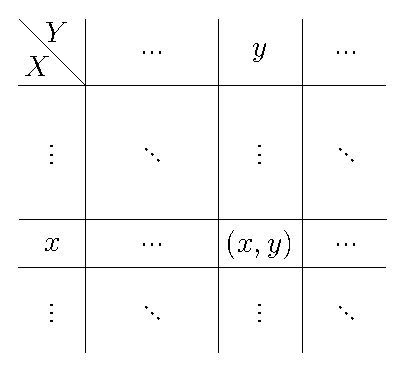
\includegraphics[width=0.25\textwidth]{2_1.eps}
	\caption{Декартово произведение}
	\label{fig:2_1}
\end{figure}

\subsection*{Примеры:}

\begin{figure}[H]
	\centering
	\begin{subfigure}[c]{0.5\textwidth}
		\centering
		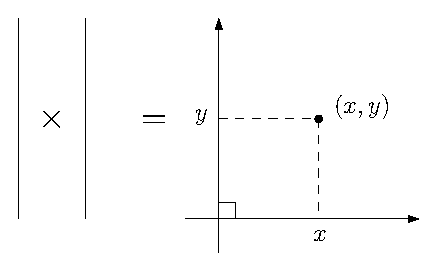
\includegraphics[width=8cm, height = 4cm]{2_2.eps}
		\caption{Прямая на прямую}
		\label{fig:2_2}
	\end{subfigure}
	\begin{subfigure}[c]{0.49\textwidth}
		\centering
		
\includegraphics[width=8cm, height = 4cm]{2_3.eps}
		\caption{Эллипс на прямую}
		\label{fig:2_3}
	\end{subfigure}
	\begin{subfigure}[c]{0.5\textwidth}
		\centering
		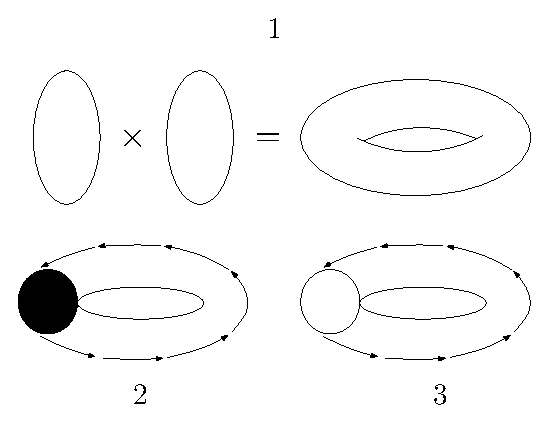
\includegraphics[width=8cm, height = 6cm]{2_4.eps}
		\caption{1: Эллипс на эллипc, 2: Полноторие, 3: Тор}
		\label{fig:2_4}
	\end{subfigure}
	\begin{subfigure}[c]{0.49\textwidth}
		\centering
		
\includegraphics[width=8cm, height = 4cm]{2_5.eps}
		\caption{Выворачивая наизнанку снова получим тор}
		\label{fig:2_5}
	\end{subfigure}
	\caption{Примеры Декартовых произведений}	
	\label{fig:Сюръективность}
\end{figure}

\begin{defn}
	Если задана $f\colon X \rightarrow Y$, то в $X\times Y$ определим подмножество $\Gamma_f = \{\,(x,y) \mid y = f(x)\,\}$ - \uwave{график функции}:
	\begin{enumerate}[label={(\arabic*)}]
		\item $\forall x \in X,\, \exists (x,y) \in \Gamma_f$ - каждому $x$ соотносится $y$;
		\item Если $(x,y) \in \Gamma_f$ и $(x,z) \in \Gamma_f$, то $y = z$;
	\end{enumerate}
\end{defn}

На языке теории множеств говорят, что задана функция из $X$ в $Y$, если задано подмножество $\Gamma \subset X\times Y$, удовлетворяющее свойствам (1)-(2).


\begin{figure}[H]
	\centering
	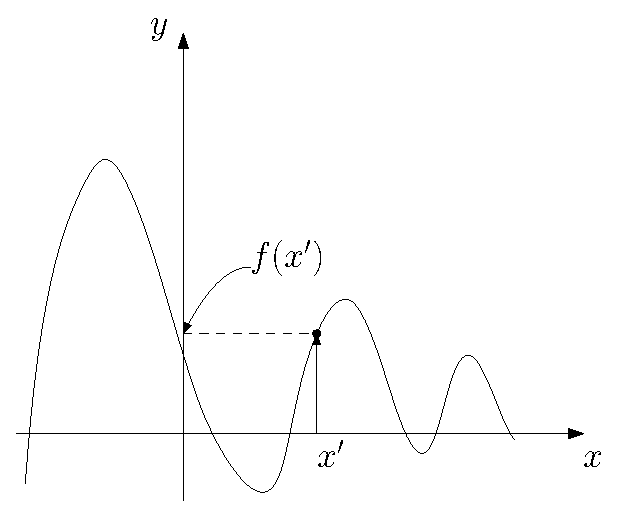
\includegraphics[width=7cm, height = 5cm]{2_6.eps}
	\caption{График функции}
	\label{fig:2_6}
\end{figure}


$\left.\begin{aligned}
	&	X \text{ - область определения функции }f & \\
	&	Y \text{ - область значения функции }f   &
\end{aligned}
\right\}
f \colon X \rightarrow Y$

\begin{defn}
	Говорят, что на множестве $X$ \uwave{задана операция} $\circ$, если задана функция из $X \times X$ в $X$,\\
	 $\circ \colon X \times X \rightarrow X$.
\end{defn}

$$(x_1,x_2) \mapsto x_1 \circ x_2$$


Операция $\circ$ на множестве $X$:
\begin{enumerate}[label={\arabic*)}]
	\item \textbf{коммутативна}, если $x_1 \circ x_2 = x_2 \circ x_1, \, \forall x_1, x_2 \in X$;
	\item \textbf{ассоциативна}, если $(x_1 \circ x_2) \circ x_3 = x_1 \circ (x_2 \circ x_3), \,\forall x_1, x_2, x_3 \in X$;
\end{enumerate}

\begin{defn}
	На множестве функций определена \uwave{операция композиций} $(f\circ g)(x) = f(g(x))$.
\end{defn}

$F(X) = \{f \mid f\colon X \rightarrow X\}$, $\circ$ - операция на $F$.

Сама операция определена для любых функций: $g \colon X \rightarrow Y$, $f\colon Y \rightarrow Z \Rightarrow f \circ g \colon X \rightarrow Z \Rightarrow$ каждому элементу из $X$ сопоставили какой-то элемент из $Z$.

\begin{rem}
	Если рассмотрим функции из множества в себя, то эта операция будет на множестве $F$.
\end{rem}

\begin{prop}
	Операция композиции ассоциативна: $(f\circ g) \circ h = f \circ (g \circ h)$.
\end{prop}

\begin{proof}
	 	$(f\circ g) \circ h (x) = \big(f\circ g\big) \big(h (x)\big) = f\Big( g\big(h(x)\big) \Big) = f \big( (g \circ h)(x) \big) = f \circ (g \circ h) (x)$
\end{proof}

При этом, $f \circ g \neq g \circ f$, например $f(x) = 3, g(x) = - 3$.

\section*{Индуктивные определения на $\mathbb{N}$}

Сначала необходимо определить $n + m, \forall n,m \in \mathbb{N}$ - это можно посмотреть в Э. Ландау: Основы/Основания математического анализа.

$n+1 = \text{след}(n) \Rightarrow \forall m \in \mathbb{N}$, зная $n+m$ имеем следующее: $n + (m+1) = (n+m) + 1$.

\begin{prop}
	$\forall n \in \mathbb{N},\, \exists!$ функция $f_n \colon \mathbb{N} \rightarrow \mathbb{N}$, такая что:
	\begin{enumerate}[label={(\arabic*)}]
		\item $f_n(1) = n + 1$;
		\item $f_n(m+1) = f_n(m) + 1$;
	\end{enumerate}
\end{prop}

\begin{defn}
	$n + m = f_n(m)$
\end{defn}

\begin{proof}
	\textbf{(единственность)} пусть таких функций 2: $f_n$ и $g$, $f_n(1) = g(1) = n+1$, $f_n(m+1) = f_n(m) + 1$, $g(m+1) = g(m) + 1$. Докажем по индукции, что $f_n = g \colon f_n(m) = g(m),\, \forall m$.\\
	\uline{База}: $m=1 \Rightarrow $ ok.\\
	\uline{Шаг}: пусть $g(m) = f_n(m)$, то $f_n(m+1) = f_n(m) + 1 = g(m) + 1 = g(m+1) \Rightarrow $ ok.
	
	\textbf{(существование)} по индукции относительно $n$:\\
	\uline{База}: $n=1 \Rightarrow$ возьмем $f_1(m) = m+1 \Rightarrow f_1(1) = 1 + 1 = 2$, $f_1(m+1) = \overbrace{m + 1}^{f_1(m)} + 1 = f_1(m) + 1$, отсюда вместе с этим получим и $m+1 = 1+ m$, поскольку $1 + m = f_1(m)$ - по определению, а также по единственности фукнции.\\
	\uline{Шаг}: пусть для $n$ такая функция $f_n$ уже есть, построим ее для $n+1$:\\
	Возьмем $f_{n+1}(m) = f_n(m) + 1 \Rightarrow f_{n+1}(1) = f_n(1) + 1 = (n+1) + 1$ - следующий за $n+1 \Rightarrow$ ok.\\
	$f_{n+1}(m+1) = f_n(m+1) + 1 = (f_n(m) + 1) + 1 \overset{\text{по опр.}}{=} f_{n+1}(m) + 1 \Rightarrow f_n$ - существует для любого $n$.
\end{proof}


\begin{exrc}
	Доказать, что 
	\begin{enumerate}[label={(\arabic*)}]
		\item $n + (m+ k) = (n+m) + k$ - индукцией по $k$;
		\item $n + m = m+ n$ - индукцией по $m$;
	\end{enumerate}
\end{exrc}

\begin{prop}
	$\forall n, m, k \in \mathbb{N}$ справедливо: 
	\begin{enumerate}[label={(\arabic*)}]
		\item $(n + m) + k = n + (m+k)$;
		\item $n + m = m + n$;
	\end{enumerate}
\end{prop}

\begin{proof}
	(1) индукцией по $k$:\\
	\uline{База}: $(n + m) + 1 = f_n(m) + 1 = f_n(m+1) = n + (m+1) \Rightarrow$ ok.\\
	\uline{Шаг}: Пусть верно для $k$, то есть $(n+m) + k = n + (m+k) \Rightarrow (n + m) + (k + 1) = f_{n+m}(k+1) = f_{n+m}(k) + 1 = \big((n+m) + k \big) + 1 = \big(n + (m + k) \big) + 1 = f_n\big((m+k)\big) + 1 = f_n\big((m+k) + 1\big) = n + \big((m+k) + 1 \big) = n + \big( f_m(k) + 1 \big) \overset{\text{по инд.}}{=} n + \big( f_m(k+1) \big) = n + \big(m + (k+1) \big) \Rightarrow$ ok.
	
	
	(2) индукцией по $m$:\\
	\uline{База}: $n + 1 = f_n(1)$, вместе с этим $1 + n = f_1(n) = n + 1 \Rightarrow 1 + n = n + 1 \Rightarrow$ ok.\\
	\uline{Шаг}: Пусть верно для $m$: $n + m = m + n \Rightarrow n + (m + 1) = f_n(m+1) = f_n(m) + 1 = (n + m) + 1 \overset{\text{по инд.}}{=} (m + n) + 1 = f_m(n) + 1 = f_{m + 1}(n) = (m + 1) + n \Rightarrow$ ok.
\end{proof}

Аналогично вводится умножение (используя индукцию).

$\left\{ \begin{aligned}
	& n \cdot 1 = n\\
	& n \cdot (m + 1) = n \cdot m + n
\end{aligned}
\right., \Rightarrow \text{далее проверяется ассоциативность и коммутативность.}$


\begin{defn}
	Множество \uwave{целых чисел} $\mathbb{Z} = \mathbb{N} \cup \{0\} \cup \{\,-n \mid n \in \mathbb{N}\,\}$.
\end{defn}

\begin{rem}
	Операция ``$+$'' и ``$\cdot$'' переносятся с множества $\mathbb{N}$, как в школе.
\end{rem}

\begin{defn}
	Подмножество $R \subset X\times X$ называется \uwave{отношением эквивалентности}, если выполняются следующие свойства:
	
	\begin{enumerate}[label={(\arabic*)}]
		\item $\forall x \in X$, $(x,x) \in R$ (рефлексивность);
		\item Если $(x,y) \in R$, то $(y,x) \in R$ (симметричность);
		\item Если $(x,y) \in R$, $(y,z) \in R$, то $(x,z) \in R$ (транзитивность);
	\end{enumerate}
\end{defn}

\textbf{Примеры}: (1) подобие треугольников; (2) $m>1, n\sim k; n,k \in \mathbb{Z} \Leftrightarrow n - k \divby m$.
\newpage
\section*{Классы эквивалентностей}

\begin{defn}
	$R(a) = \{\,x \mid x \sim a\,\}$ - называется \uwave{классом эквивалентностей с представителем $a$}.
\end{defn}

\begin{prop}
	Если $R(a) \cap R(b) \neq \varnothing \Rightarrow R(a) = R(b)$.
\end{prop}

\begin{proof}
	Пусть $c \in R(a) \cap R(b) \Rightarrow a \sim c \wedge b \sim c \Leftrightarrow a \sim c \wedge c \sim b \Rightarrow a \sim b \Rightarrow \forall x \sim b \Rightarrow x \sim a$\\
	$\forall x \sim a \Rightarrow x \sim b \Rightarrow R(a) = R(b)$.
\end{proof}

\begin{defn}
	\uwave{Разбиение множества $A$} - набор непустых подмножеств множества $A$, таких что объединение этих подмножеств дает $A$, причем подмножества попарно не пересекаются. 
\end{defn}

\begin{theorem}
	Пусть $R$ - отношение эквивалентности на множестве $X$. Множество $\{\,R(x) \mid x \in X\,\}$ - классов эквивалентности формируют разбиение множества $X$.
\end{theorem}

\begin{proof}
	$R(x) \neq R(y) \Rightarrow R(x) \cap R(y) = \varnothing \Leftrightarrow \big(R(x) \cap R(y) \neq \varnothing \Rightarrow R(x) = R(y)\big)$.\\
	Пусть $\tilde{x} \in \bigcup\limits_{x \in X} R(x) \Rightarrow \exists y \in X \colon \tilde{x} \in R(y); R(y) \subseteq X \Rightarrow \tilde{x} \in X \Rightarrow \bigcup\limits_{x \in X} R(x) \subseteq X$.\\
	Пусть $z \in X, z \in R(z) \Rightarrow z \in R(y)$, для некоторых $y \in X \Rightarrow z \in \bigcup\limits_{x \in X} R(x) \Rightarrow X \subseteq \bigcup\limits_{x \in X} R(x)$. \\
	$\Rightarrow X = \bigcup\limits_{x \in X} R(x)$. 
\end{proof}

Таким образом $\{\,R(x) \mid x \in X\,\}$ - разбиение множества $X$.

\begin{defn}
	Набор классов эквивалентности называется \uwave{фактор-множеством} $X/\sim$.
\end{defn}

Рассмотрим $\mathbb{Z}\times \mathbb{N}: (m,n) \sim (p,q) \Leftrightarrow mq = pn, m \in \mathbb{Z}, n \in \mathbb{N}$. В данном контексте $(m,n)$ и $(p,q)$ можно рассматривать, как $\frac{m}{n}$ и $\frac{p}{q}$.

\begin{defn}
	Множество классов эквивалентностей, заданных таким образом, называется \uwave{множеством рациональных чисел} или дробей и обозначается $\mathbb{Q}$.
\end{defn}


\end{document}